\documentclass[border=0in]{standalone}

\usepackage[T1]{fontenc}
\usepackage{opensans}
\usepackage{bm}
\usepackage{mathrsfs}

\usepackage{tikz}
\usepackage{pgfplots}
\pgfplotsset{compat=1.18}
\usepackage{amsmath}
\usepackage{amsfonts}
\usepackage{amssymb}
\usepackage{xcolor}
\usepackage{newtxsf}

\usepgfplotslibrary{fillbetween}

\definecolor{c0}{HTML}{f0f9e8}
\definecolor{c1}{HTML}{bae4bc}
\definecolor{c2}{HTML}{7bccc4}
\definecolor{c3}{HTML}{43a2ca}
\definecolor{c4}{HTML}{0868ac}
\definecolor{lightgray}{HTML}{d3d3d3}
\newcommand{\grtr}{\natural}


\begin{document}

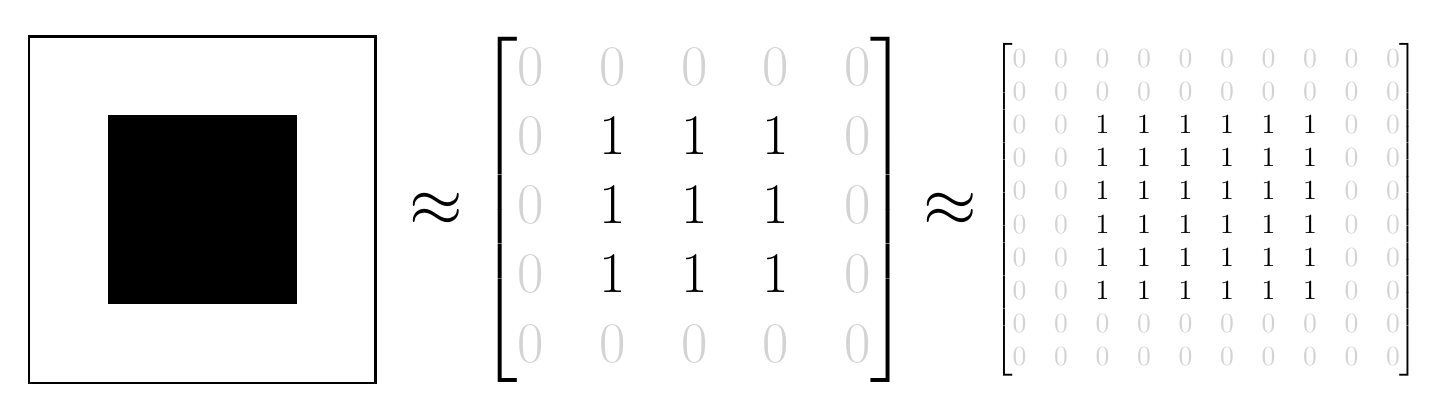
\begin{tikzpicture}

  % bounding box
  \draw[black, fill=white, line width=1pt] (-2.2,-2.2) rectangle (2.2,2.2); % Adjust the dimensions as needed
  
  % Black Square
  \fill[black] (-1.2,-1.2) rectangle (1.2,1.2); % Adjust the coordinates to position the square

  % first approx sign
  \node [anchor=center] at (2.97, 0) {{\Huge $\approx$ }};


  % discretized matrix
  \node [anchor=center] at (6.25, 0) {{\huge $\begin{bmatrix}
          {\color{lightgray} 0} && {\color{lightgray} 0} && {\color{lightgray}
          0} && {\color{lightgray} 0} && {\color{lightgray} 0} \\
          {\color{lightgray} 0} && 1 && 1 && 1 && {\color{lightgray} 0} \\
          {\color{lightgray} 0} && 1 && 1 && 1 && {\color{lightgray} 0} \\
          {\color{lightgray} 0} && 1 && 1 && 1 && {\color{lightgray} 0} \\
          {\color{lightgray} 0} && {\color{lightgray} 0} && {\color{lightgray}
          0} && {\color{lightgray} 0} && {\color{lightgray} 0}
  \end{bmatrix}$}};


  % second approx sign
  \node [anchor=center] at (9.5, 0) {{\Huge $\approx$ }};


  % discretized matrix 2
  \node [anchor=center] at (12.75, 0) { $\begin{bmatrix}
  \begin{matrix}
    \color{lightgray} 0 & \color{lightgray} 0 \\
    \color{lightgray} 0 & \color{lightgray} 0 \\
  \end{matrix} & \begin{matrix}
    \color{lightgray} 0 & \color{lightgray} 0 \\
    \color{lightgray} 0 & \color{lightgray} 0 \\
  \end{matrix} & \begin{matrix}
    \color{lightgray} 0 & \color{lightgray} 0 \\
    \color{lightgray} 0 & \color{lightgray} 0 \\
  \end{matrix} & \begin{matrix}
    \color{lightgray} 0 & \color{lightgray} 0 \\
    \color{lightgray} 0 & \color{lightgray} 0 \\
  \end{matrix} & \begin{matrix}
    \color{lightgray} 0 & \color{lightgray} 0 \\
    \color{lightgray} 0 & \color{lightgray} 0 \\
  \end{matrix} \\
  
  \begin{matrix}
    \color{lightgray} 0 & \color{lightgray} 0 \\
    \color{lightgray} 0 & \color{lightgray} 0 \\
  \end{matrix} & \begin{matrix}
    1 & 1 \\
    1 & 1 \\
  \end{matrix} & \begin{matrix}
    1 & 1 \\
    1 & 1 \\
  \end{matrix} & \begin{matrix}
    1 & 1 \\
    1 & 1 \\
  \end{matrix} & \begin{matrix}
    \color{lightgray} 0 & \color{lightgray} 0 \\
    \color{lightgray} 0 & \color{lightgray} 0 \\
  \end{matrix} \\
  
  \begin{matrix}
    \color{lightgray} 0 & \color{lightgray} 0 \\
    \color{lightgray} 0 & \color{lightgray} 0 \\
  \end{matrix} & \begin{matrix}
    1 & 1 \\
    1 & 1 \\
  \end{matrix} & \begin{matrix}
    1 & 1 \\
    1 & 1 \\
  \end{matrix} & \begin{matrix}
    1 & 1 \\
    1 & 1 \\
  \end{matrix} & \begin{matrix}
    \color{lightgray} 0 & \color{lightgray} 0 \\
    \color{lightgray} 0 & \color{lightgray} 0 \\
  \end{matrix} \\
  
  \begin{matrix}
    \color{lightgray} 0 & \color{lightgray} 0 \\
    \color{lightgray} 0 & \color{lightgray} 0 \\
  \end{matrix} & \begin{matrix}
    1 & 1 \\
    1 & 1 \\
  \end{matrix} & \begin{matrix}
    1 & 1 \\
    1 & 1 \\
  \end{matrix} & \begin{matrix}
    1 & 1 \\
    1 & 1 \\
  \end{matrix} & \begin{matrix}
    \color{lightgray} 0 & \color{lightgray} 0 \\
    \color{lightgray} 0 & \color{lightgray} 0 \\
  \end{matrix} \\
  
  \begin{matrix}
    \color{lightgray} 0 & \color{lightgray} 0 \\
    \color{lightgray} 0 & \color{lightgray} 0 \\
  \end{matrix} & \begin{matrix}
    \color{lightgray} 0 & \color{lightgray} 0 \\
    \color{lightgray} 0 & \color{lightgray} 0 \\
  \end{matrix} & \begin{matrix}
    \color{lightgray} 0 & \color{lightgray} 0 \\
    \color{lightgray} 0 & \color{lightgray} 0 \\
  \end{matrix} & \begin{matrix}
    \color{lightgray} 0 & \color{lightgray} 0 \\
    \color{lightgray} 0 & \color{lightgray} 0 \\
  \end{matrix} & \begin{matrix}
    \color{lightgray} 0 & \color{lightgray} 0 \\
    \color{lightgray} 0 & \color{lightgray} 0 \\
  \end{matrix}
\end{bmatrix}$};

  % \node [anchor=center] at (6, 0) {$abcd$};


\end{tikzpicture}

\end{document}
